\documentclass[10pt]{article}
\usepackage{../../local}
\urlstyle{same}

\newcommand{\classcode}{Physics C191}
\newcommand{\classname}{Introduction to Quantum Information}
\renewcommand{\maketitle}{%
\hrule height4pt
\large{Eric Du \hfill \classcode}
\newline
\large{HW 07} \Large{\hfill \classname \hfill} \large{\today}
\hrule height4pt \vskip .7em
\small{Header styling inspired by CS 70: \url{https://www.eecs70.org/}}
\normalsize
}
\linespread{1.1}
\begin{document}
	\maketitle
	\section*{Problem 1}
	Suppose we have 3 identical physical qubits that experience exponential longitudinal relaxation with 
	\( 1 / e \) lifetimes of \( T_1 = 1 / \gamma \) for each of the qubits so that the probability of error 
	on a single qubit \( p(t) = 1 - e^{- \gamma t} \), which may be approximated to lowest non-zero order 
	as \( p(t) = \gamma t \). (For the sake of simplicity we will assume that the 
	relaxation process is symmetric with respect to \( \ket*{0} \) and \( \ket*{1} \)). We use the 
	three-qubit bit-flip error correction code you learned about in lecture (see below) to encode a single logical 
	qubit, \( \ket*{\psi}_i \), in the three physical qubits, wait for time \( t \), and decode 
	it to get \( \ket*{\psi}_f \). 

	\textit{Note:} For the entire problem, you can assume perfect initial state preparation at the start of the circuit,
	and instantaneous and error free gates throughout the circuit. 
	\begin{center}
		\begin{quantikz}
			\lstick{\( \ket*{\psi}_i \) } & \ctrl{1} & \ctrl{2} & \gate[3]{\text{Evolution for time $t$}} & 
			\ctrl{1} & \ctrl{2} & \targ{} & \rstick{\( \ket*{\psi}_f \) }\\
			\lstick{\( \ket*{0} \) } & \targ{} & & & \targ{} & & \ctrl{-1} & \\
			\lstick{\( \ket*{0} \) } & &\targ{} & & & \targ{} & \ctrl{-2} & 
		\end{quantikz}
	\end{center}
	\begin{enumerate}[label=\alph*)]
		\item To lowest nonzero order, at approximately what wait time \( t \) would a single unencoded physical 
			qubit have a 1\% probability of experiencing a bit-flip error?

			\begin{solution}
				To start, we can show that our initial qubit is in the state:
				\[
				\ket*{\psi} = a\ket*{000} + b \ket*{111}
				\] 
				We're given that we should use \( p(t) = \gamma t \) here, so this means that if we want a 
				1\% probability error, then we want:
				\[
				p(t) = \frac{1}{100} \implies t = \frac{1}{100\gamma}
				\] 
			\end{solution}
		\item To lowest nonzero order, at approximately what wait time \( t \) would the logical qubit 
			(before decoding) have a 1\% probability of experiencing a bit-flip error?

			\begin{solution}
				Since this is a three qubit repetition code, then there are three places that our bit-flip could 
				happen. Therefore, the probability of a bit-flip is \( 3p(t) = 3\gamma t \), so:
				\[
				3\gamma t = \frac{1}{100} \implies t = \frac{1}{300 \gamma}
				\] 
				This \( t \) is smaller than that of the previous part, which makes intuitive sense since we have 
				thrice the probability of having an error. 
			\end{solution}
		\item To lowest nonzero order, at approximately what wait time \( t \) will the corrected 
			logical state (after decoding)  \( \ket*{\psi}_f \) have a 1\% probability of having experienced 
			a bit-flip error?

			\begin{solution}
				To lowest-order, this would occur when we have two bit flips happen simultaneously. Firstly, there 
				are three ways that two bit flips could happen: \( (1, 1, 0), (1, 0, 1), (0, 1, 1) \). Therefore, 
				the probability of a bit flip is given by \( 3(p(t))^2 = 3\gamma^2 t^2\), so therefore:
				\[
				3\gamma^2 t^2 = \frac{1}{100} \implies t = \frac{1}{3 \gamma \sqrt{100}}
				\] 
			\end{solution}
		\item At what wait time \( t \) will the probability of a single physical qubit bit-flip error be equal 
			to the probability of a bit-flip error on the decoded state \( \ket*{\psi}_f \)? 

			\begin{solution}
				The probability of a single bit-flip error is \( p(t) = 1 - e^{-\gamma t} \), and the probability 
				of a logical error is \( 3(1 - e^{- \gamma t})^2 \), so setting them equal:
				\begin{align*}
					1 - e^{-\gamma t} &= 3(1 - e^{-\gamma t})^2\\
					e^{-\gamma t} &=  \frac{2}{3} \\
					\therefore t &= -\frac{1}{\gamma} \ln\left( \frac{2}{3} \right)  
				\end{align*}
			\end{solution}
		\item If we define the \( T_{1, L} \) lifetime of the encoded logical qubit \( \ket*{\psi}_f \) in the 
			same manner as for a single qubit, meaning \( T_{1, L} \) is the time at which the probability 
			for \( \ket*{\psi}_f \) to \textit{not} have experienced a bit-flip is equal to \( 1 / e \), 
			then is  \( T_{1, L} \) longer or shorter than the single qubit lifetime \( T_1 \)?

			\begin{solution}
				This problem basically asks us to find the time \( t \) such that:
				\[
				3(1 - e^{-\gamma t})^2 = 1 - \frac{1}{e} \implies T_{1, L} = -\frac{1}{\gamma}
				\ln\left( 1 - \sqrt{\frac{1}{3}(1 - e^{-1}) }\right) 
				\] 
				whereas for a single qubit, we have \( T_1 = \frac{1}{\gamma} \). The factor attached 
				to the \( \frac{1}{\gamma} \) in the above expression is equal to \( -0.61 \), meaning that 
				\( T_{1, L} \) is shorter than \( T_1 \).  

				This also makes sense, since the probability of having a logical bit flip is higher than 
				the probability of a single bit flip, so we expect the lifetime to be shorter. 
			\end{solution}
	\end{enumerate}
	\pagebreak
	\section*{Problem 2}
	This question will help you understand Pauli commutation relations, an important part of 
	syndrome extraction analysis. First, we summarize a convenient and standard short-hand notation 
	for \( n \)-qubit Pauli operators: subscript the non-trivial Pauli operators (i.e. \( X, Y, Z \) excluding
	\( I \)) with the qubit on which they act. For example, on 5-qubits and indexing 
	the first qubit at 1, \( X_1 = X \otimes I \otimes I \otimes I \otimes I \), 
	\( X_1X_2 = X \otimes X \otimes I \otimes I \otimes I \), \( X_2Y_4 = I \otimes X \otimes I \otimes Y \otimes I\),
	etc\dots

	Recall that two operators, \( F_i \) and \( F_j \) commute if \( F_i F_j = F_j F_i \), and anti-commute 
	if \( F_iF_j = (-1)F_jF_i \). consider a register of 8 qubits. Do the following pairs of operators commute or 
	anti-commute? Show your work and/or explain your reasoning. 
	\begin{enumerate}[label=\alph*)]
		\item \( X_1, Y_1 \).

			\begin{solution}
				I'm using the relations given in discussion section. There we mentioned that 
				\( X_1 Z_1 = - Z_1 X_1 \), since they act on the the same qubit. The same logic applies here, 
				so since both subscripts are 1, then these two anticommute. 
			\end{solution}
		\item \( Z_1Z_2, Y_1Y_2 \) 

			\begin{solution}
				Here, we are asked to compare the operators \( Z_1Z_2 Y_1 Y_2 \) against \( Y_2Y_1 Z_2Z_1 \), which 
				do commute:
				\[
				Y_1Y_1Z_2Z_1 = (-1)Z_2Y_2 (-1)Z_1Y_1 = Z_2Y_2Z_1Y_1 = Z_2Z_1Y_2Y_1 = Z_1Z_2 Y_1Y_2
				\] 
			\end{solution}
		\item \( Z_1X_3Y_4, Y_1Z_2Y_4 \) 

			\begin{solution}
				These operators anticommute:
				\begin{align*}
					Y_4Z_2Y_1Y_4X_3Z_1 &= (-1)Z_1Y_4Z_2 Y_1Y_4X_3 \\
					&= (-1) Z_1X_3Y_4Z_2Y_1Y_4 \\
					&= (-1)Z_1X_3Y_4Y_1Z_2Y_4 \\
				\end{align*}
			\end{solution}
		\item \( Z_1X_2Y_3Y_5Z_6X_7Y_8 \), \( X_1X_2Z_3Z_4Y_5Z_7X_8 \)

			\begin{solution}
				We can do the math out for this, but notice a pattern in the previous two solutions: we look at the 
				operations on each qubit, and tally up the commutativity of each one:
				\begin{center}
					\begin{tabular}{c|c|c}
						Qubit & Operators & Commutativity\\
						1 & \( Z_1, X_1 \) & \( -1 \) \\
						2 & \( X_2, X_2 \) & \( 1 \)\\
						3 & \( Y_3, Z_3 \) & \( -1 \) \\
						4 & \( I, I \) & 1\\
						5 & \( Y_5, Y_5 \) & \( 1 \) \\
						6 & \( Z_6, I \) & \( 1 \) \\
						7 & \( X_7, Z_7 \) & \( -1 \) \\
						8 &  \( Y_8, X_8 \) & \( -1 \)
					\end{tabular}
				\end{center}
				Here, we see that there are an even number of anticommuting operators, so therefore this pair 
				of operators commute. 
			\end{solution}
	\end{enumerate}
	\pagebreak
	\section*{Problem 3}
	This question will have you analyze properties of the 9-qubit Shor code. For convenience, its logical states and 
	its stabilizers are provided below. 

	Logical states for the 9-qubit Shor code:
	\begin{align*}
		\ket*{0}_L &= \frac{1}{2\sqrt{2} }(\ket*{000} + \ket*{111})(\ket*{000} + \ket*{111})(\ket*{000} + \ket*{111})\\
		\ket*{1}_L &= \frac{1}{2\sqrt{2} }(\ket*{000} - \ket*{111}) (\ket*{000} - \ket*{111})(\ket*{000} - \ket*{111}) \\
	\end{align*}
	Stabilizers of the 9-qubit Shor code:
	\begin{center}
		\begin{tabular}{c|c}
			\( X_1X_2X_3X_4X_5X_6 \) & \( X_4X_5X_6X_7X_8X_9 \) \\
			\( Z_1Z_2 \) & \( Z_2Z_3 \) \\
			\( Z_4Z_5 \) & \( Z_5Z_6 \) \\
			\( Z_7Z_8 \) & \( Z_8Z_9 \)
		\end{tabular}
	\end{center}
	\begin{enumerate}[label=\alph*)]
		\item Show that the 9-qubit Shor code is distance 3. That is, show that a three qubit error 
			can take one codeword to the other codeword. 

			\begin{solution}
				From lecture, we define the distance \( d \) to be the smallest weight logical operator that 
				takes \( \ket*{0}_L \) to \( \ket*{1}_L \). It is then distance 3 because the operator
				\( Z_1Z_4Z_7 \) does precisely that. 
			\end{solution}
		\item What are the syndromes of the following errors: \( Z_1, Z_2, Z_3 \)?

			\begin{solution}
				Because the \( Z \) errors only anticommute wtih \( X \), then we only need to look at the 
				first two stabilizers in the first row:
				\begin{center}
					\begin{tabular}{c|c|c|c}
						& \( Z_1 \) & \( Z_2 \) & \( Z_3 \) \\
						\hline
						\( X_1X_2X_3X_4X_5X_6 \) & \( -1 \) & \( -1 \) &\(  -1 \) \\
						\hline
						\( X_4X_5X_6X_7X_8X_9 \) & \( 1 \) &  \( 1 \) &  \( 1 \) \\
					\end{tabular}
				\end{center}
				All the other stabilizers will be just 1 because \( Z_i \) commutes with them.   
			\end{solution}
		\item What is the effect of the \( Z_1, Z_2 \) and \( Z_3 \) on the logical states of the Shor code? 
			Provide a single correction operation that can correct each of the three individual error processes. 
			This provides an example of why the Shor code is ``degenerate," some of the errors in the set of 
			correctable errors map to the same syndrome string.

			\begin{solution}
				Because the \( Z \) error only flips the sign on the \( \ket*{1} \) state, this means that 
				all three errors send the states as follows:
				\begin{align*}
					\ket*{0}_L &\to \frac{1}{2\sqrt{2} }(\ket*{000} - \ket*{111})(\ket*{000} + \ket*{111})
				(\ket*{000} + \ket*{111})\\
					\ket*{1}_L & \to \frac{1}{2\sqrt{2} }(\ket*{000} + \ket*{111})(\ket*{000} - \ket*{111})
					(\ket*{000} - \ket*{111})
			\end{align*} 
			what this means is that we just need to flip the sign back, whihc we can do with a simple \( Z_1 \) 
			gate. 
			\end{solution}
	\end{enumerate}

	\pagebreak
	\section*{Problem 4}
	This question will have you investigate properties of the 7-qubit Steane code. For your convenience, the 
	Stabilizers are given below in a useful geometric mnemonic in the figure below. The stabilizers are denoted as 
	\( S_{x / z}^{(i)} \) for \( i \in [1, 3] \) and there are 6 in total. 
	\begin{center}
		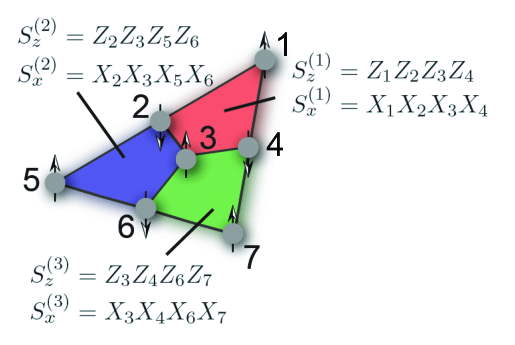
\includegraphics[scale=0.4]{q3c.png}
	\end{center}
	\begin{enumerate}[label=\alph*)]
		\item Tabulate the syndromes of all single qubit \( Z \)-type errors of the form \( Z_i \) for \( i \) in the 
			range \( [1, 7]\). Please use syndrome ordering so that the associated stabilizers appear in the order 
			\( S_x^{(1)}, S_x^{(2)}, S_x^{(3)}, S_z^{(1)}, S_z^{(2)}, S_z^{(3)} \). 

			\begin{solution}
				Here's the table:
				\begin{center}
					\begin{tabular}{c|c|c|c|c|c|c|c}
						&  \( Z_1 \) & \( Z_2 \) & \( Z_3 \) & \( Z_4 \) & \( Z_5 \) & \( Z_6 \) & \( Z_7 \) \\
						\( S_x^{(1)} \) & \( -1 \) & \( -1 \) & \( -1 \) & \( -1 \) & \( 1 \) & \( 1 \) & $1$ \\
						\( S_x^{(2)} \) & \( 1 \) & \( -1 \) &  \( -1 \) & \( 1 \) & \( -1 \) & \( -1 \) & \( 1 \) \\
						\( S_x^{(3)} \) & \( 1 \) & \( 1 \) & \( -1 \) &  \( -1 \) & \( 1 \) & \( -1  \) & \( -1 \)\\
						\( S_z^{(1)} \) & \( 1 \) & \( 1 \) & \( 1 \) & \( 1 \) & \( 1 \) & \( 1 \) & \( 1 \)\\
						\( S_z^{(2)} \) & \( 1 \) & \( 1 \) & \( 1 \) & \( 1 \) & \( 1 \) & \( 1 \) & \( 1 \)\\
						\( S_z^{(3)} \) & \( 1 \) & \( 1 \) & \( 1 \) & \( 1 \) & \( 1 \) & \( 1 \) & \( 1 \)
					\end{tabular}
				\end{center}
			\end{solution}
		\item Tabulate the syndromes of all single qubit \( X \)-type errors of the form \( X_i \) for 
			\( i \) in the range \( [1, 7] \). Please use the same syndrome ordering as in part (a). 

			\begin{solution}
				Again, here's the table:
					\begin{center}
					\begin{tabular}{c|c|c|c|c|c|c|c}
						&  \( X_1 \) & \( X_2 \) & \( X_3 \) & \( X_4 \) & \( X_5 \) & \( X_6 \) & \( X_7 \) \\
						\( S_x^{(1)} \) & \( 1 \) & \( 1 \) & \( 1 \) & \( 1 \) & \( 1 \) & \( 1 \) & \( 1 \)\\
						\( S_x^{(2)} \) & \( 1 \) & \( 1 \) & \( 1 \) & \( 1 \) & \( 1 \) & \( 1 \) & \( 1 \)\\
						\( S_x^{(3)} \) & \( 1 \) & \( 1 \) & \( 1 \) & \( 1 \) & \( 1 \) & \( 1 \) & \( 1 \)\\
						\( S_z^{(1)} \) & \( -1 \) & \( -1 \) & \( -1 \) & \( -1 \) & \( 1 \) & \( 1 \) & $1$ \\
						\( S_z^{(2)} \) & \( 1 \) & \( -1 \) &  \( -1 \) & \( 1 \) & \( -1 \) & \( -1 \) & \( 1 \) \\
						\( S_z^{(3)} \) & \( 1 \) & \( 1 \) & \( -1 \) &  \( -1 \) & \( 1 \) & \( -1  \) & \( -1 \)
					\end{tabular}
				\end{center}
			\end{solution}
		\item How many errors are there of the form 
			\[
			Z_i^{a}X_j^{b} 
			\] 
			for \( a \in \{0, 1\} , b \in \{0, 1\} , i \in [1, 7], j \in [1, 7] \)?

			\begin{solution}
				We only get an error if either one of  \( a, b = 1 \), and there are seven options of choosing 
				which qubit this error occurs to, and one option of not choosing a qubit at all. Therefore, there are 
				\( 8 \times 8 = 64 \) total errors. (this includes the case where we have no error as well)
			\end{solution}
		\item How many unique syndromes are there in the Steane code? 

			\begin{solution}
				There are six stabilizers, meaning that our error space is size \( 2^{6} = 64 \), which is precisely 
				the number of unique syndromes. 
			\end{solution}
		\item Argue that the Steane code can correct all errors of the form 
			\[
			Z_i^{a}X_j^{b}
			\] 
			and no more (you may use the fact that the Steane code is non-degenerate).

			\begin{solution}
				Because the number of unique syndromes equals the number of unique errors, along with the fact that 
				the Steane code is non-degenerate, this implies that there is a bijection between every error 
				of the above form and its corresponding syndrome. This means that given any syndrome, we can 
				automatically determine which weight-2 error caused it, and hence we can correct for it. 

				It also cannot correct for any more errors than this, since any other introduced error would 
				have an identical syndrome to one of the weight-2 errors, and hence it is no longer correctable.  
			\end{solution}
	\end{enumerate}
\end{document}
